\section{Theoretical Background} \label{sec:theory}
The purpose of this chapter is to go through the basic wind turbine (WT) theory. 

\subsection{Aerodynamics and airfoil theory}
The sun delivers energy to the earth by heating up the surface and subsequently the air of the earth. Winds occur as a result of the pressure differences that occur due to the expansion and contraction of the air. \\

WTs work because they are able to convert the wind's energy into a torque in the generator which then generates electrical energy. When the wind blows over the blades of a WT it delivers some of its energy to the blade, yielding both a thrust force and torque to the blade.

In the simplest 1D momentum theory case the delivery of energy just results in a lowing of the wind speed following the rotor area. Due to mass retention an expansion would subsequently occur as seen in \cref{fig:betz}.
\begin{figure}[h]
	\centering
	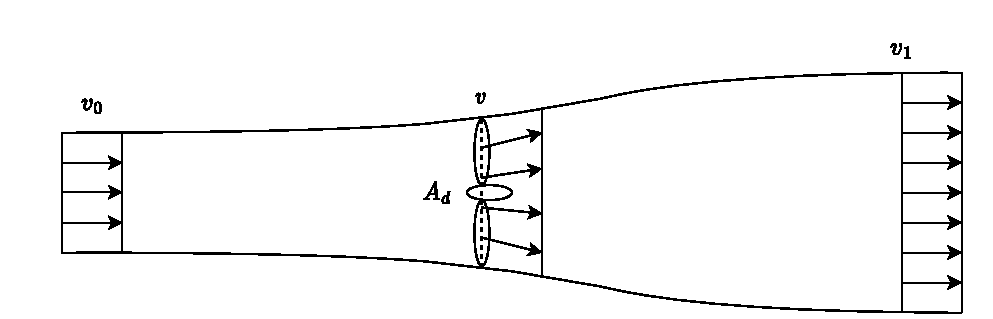
\includegraphics[width=0.8\linewidth]{Graphics/FlowThroughRotor.pdf}
	\caption{Illustration of how the wind in a control volume (CV) changes volume due to its reduction of speed}
	\label{fig:betz}
\end{figure}
The energy in the wind can be expressed as kinetic energy:
\begin{equation} \label{eq:energy}
	E = \dfrac{1}{2} m v_0^2
\end{equation}
Subsequently the power can be calculated as the time derivative of the energy:
\begin{equation} \label{eq:power}
	P = \dot{E} = \dfrac{1}{2} \dot{m} v_0^2
\end{equation}
The time derivative of the mass can be expressed from the air density $ \rho $, the cross-sectional area $ A_d $ and the wind velocity $ v_0 $:
\begin{equation}\label{eq:mass_deriv}
	\dot{m} = \rho A_d v_0
\end{equation}
Combining \cref{eq:mass_deriv} and \cref{eq:mass_deriv} yields:
\begin{equation}\label{eq:power2}
	P_{air} = \dfrac{1}{2} \rho A_d v_0^3
\end{equation}
A \textit{power coefficient} $ C_p $ is used to represent the percentage of the available power that is extracted from the wind:
\begin{equation}\label{eq:power_w_Cp}
	P_{T} = \dfrac{1}{2} \rho A_d v_0^3 C_p
\end{equation}
$ C_p $ is dependent on the rotor blade pitch $ \theta $ and the tip speed ratio $ \lambda $. In some of the operating range of a WT the goal is to reach an optimal $ C_p $ by adjusting $ \theta $ and  $ \lambda $ to their optimal values:
\begin{equation}\label{eq:cp_optimal}
	C_p^\star = C_p(\theta^\star, \lambda^\star)
\end{equation}
 The achievable size of $ C_p^\star $ is a matter of the WT design. The \textit{Betz limit} is the highest, optimal $ C_p $ that can be theoretically achieved and can be calculated to be:
\begin{equation}\label{eq:betzlimit}
	C_{pbetz} = 0.5962
\end{equation}
Thus efficiency is calculated from the Betz limit:
\begin{equation}\label{eq:efficiency}
	\eta = \dfrac{C_p}{C_{pbetz}}
\end{equation}

When the air travels over the WT blade the air travels slower on one side than the other as illustrated in \cref{fig:airfoil}. Due to mass conservation the air which moves slower on the underside of the blade expands, creating a higher pressure. Likewise the air moving faster on the upper upper side contracts creating in a lower pressure. Resultingly the blade moves upwards.
\begin{figure}[h]
	\centering
	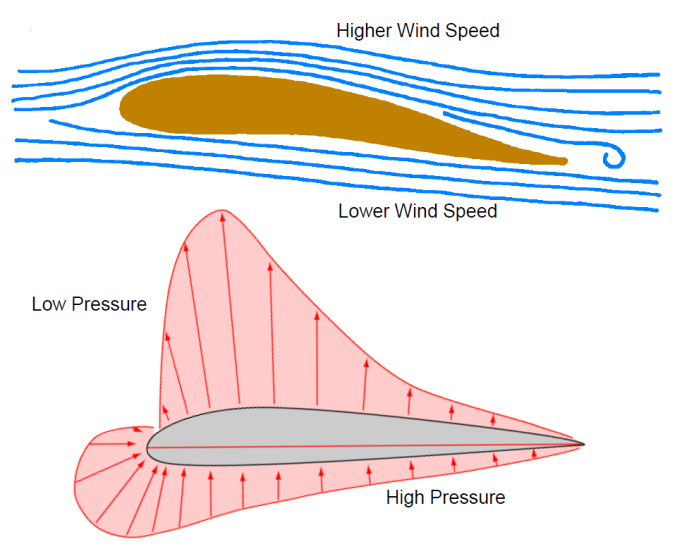
\includegraphics[width=0.5\linewidth]{Graphics/AirfoilAirflow.png}
	\caption{Illustration of the wind speed difference between the two sides of a WT blade along with an illustration of the induced pressure difference. The result is a lifting force one the blade.}
	\label{fig:airfoil}
\end{figure}
Blade element momentum theory is often used to model the forces acting along WT blades. Blade element theory involves breaking a blade into small sections and determining the forces acting on that section. In \cref{fig:blade_vel_triangle} a cross section of a WT blade can be seen. In this figure, as it is also illustrated at the rotor blade in \cref{fig:betz}, the wind velocity that hits the rotor blades is lowered indicated by the \textit{axial induction factor} $ a $. What is not observed in \cref{fig:betz} is that some of the energy of the wind also goes into driving an airstream around the back of the rotors in the opposite direction of the blade rotation, indicated by the \textit{tangential induction factor} $ a' $. This is known as \textit{swirl losses}.

\begin{figure}[h]
	\centering
	\begin{subfigure}[t]{.44\textwidth}
		\centering
		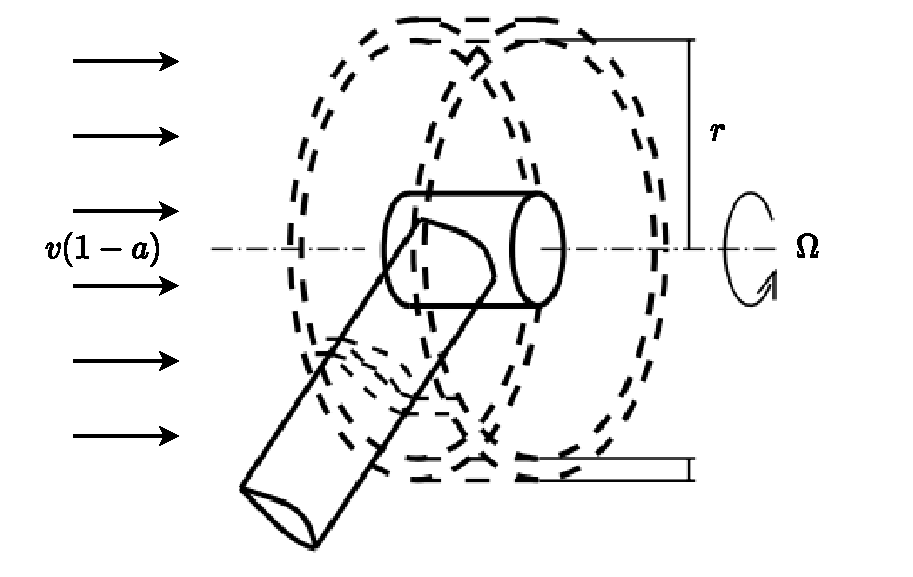
\includegraphics[width=1\linewidth]{Graphics/RotorBladeElement.pdf}
		\caption{Illustration of a blade cross section}
		\label{fig:blade_vel_triangles}
	\end{subfigure}%
	\hspace{0.01cm}
	\begin{subfigure}[t]{.55\textwidth}
		\centering
		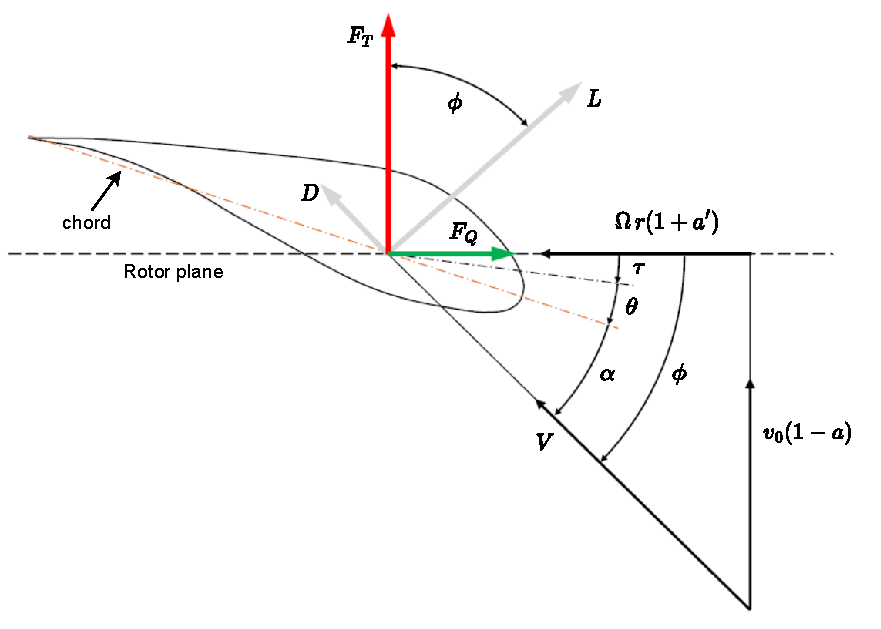
\includegraphics[width=1\linewidth]{Graphics/BladeVelocityTriangle.pdf}
		\caption{Velocity triangle with the rotation induction factor $ a' $ included \textbf{TO DO: Ensret notation ift. om vindhastighed er U eller v!}}
		\label{fig:blade_vel_triangle}
	\end{subfigure}
	
	\caption{Illustrations of the velocity triangle acting on a cross section of a WT blade}
	\label{fig:blade_triangles}
\end{figure}

The resulting air speed is V with an \textit{inflow angle} $ \phi $. $ L $ and $ D $ is the lift and drag forces respectively. They are calculated from \cref{eq:lift} and \cref{eq:drag}. They include the \textit{chord length} $ c $ which is the length from the leading to the trailing edge of the blade and $ \phi $.
\begin{align}
	L &= \dfrac{1}{2} \rho V^2 c \, C_L \label{eq:lift}\\
	D &= \dfrac{1}{2} \rho V^2 c \, C_D \label{eq:drag}
\end{align}
The lift and drag coefficients $ C_L $ and $ C_D $ are usually extracted from table lookups which are typically found from simulations such as Xfoil \textbf{TO DO: Find ud af hvad Vestas bruger til at udregne disse coefficienter!}. In a typical scenario $ C_L $ is found from the angle of attack $ \alpha $ and $ C_D $ is subsequently found from $ C_L $.